%% ===================================================================
%% QSS 20 final paper -- draft
%%
%% PORTING TO THE PNAS TEMPLATE (do this before submitting):
%%   1. Open the PNAS Overleaf gallery, take the *single-column
%%      mathematics article* template (2nd from left), "Open as Template".
%%   2. In pnas-new.cls set the DRAFT watermark to false.
%%   3. Upload output/fig1-3.png and output/table1-4.tex into the
%%      Overleaf project, then set \OUT below to {.} (see next line).
%%   4. Paste everything between \begin{document} and \end{document}
%%      into the template body. Section names map one-to-one.
%%
%% This preamble only exists so the draft compiles locally; the PNAS
%% class replaces it entirely.
%% ===================================================================
\documentclass[9pt]{extarticle}
\usepackage[letterpaper,margin=0.9in]{geometry}
\linespread{1.02}
\usepackage{graphicx}
\usepackage{booktabs}
\usepackage{amsmath}
\usepackage{caption}
\usepackage{xcolor}
\usepackage[colorlinks=true,allcolors=blue]{hyperref}
\captionsetup{font=small,labelfont=bf}
\setlength{\parskip}{0pt}
\setlength{\textfloatsep}{10pt plus 2pt minus 2pt}
\setlength{\intextsep}{10pt plus 2pt minus 2pt}
\setlength{\abovecaptionskip}{5pt}

%% path to the generated figures and tables; set to {.} on Overleaf
\newcommand{\OUT}{../output}
\graphicspath{{../output/}{./}}


\title{\vspace{-2em}Which Rural Places Move Kids Up?\\
\large Neighborhood Correlates of Upward Mobility Within Rural Labor Markets}
\author{Maxwell Fortner\\\small Dartmouth College, QSS 20}
\date{\small\today}

\begin{document}
\maketitle

\begin{abstract}
\noindent Research on neighborhoods and intergenerational mobility is
overwhelmingly urban, and the Opportunity Atlas notes that rurality helps
children in some regions and hurts them in others without saying what separates
the two. I ask which neighborhood characteristics distinguish rural Census
tracts with above-average upward mobility from otherwise similar rural tracts.
Comparing
17{,}310 rural tracts to other tracts inside the same commuting zone, the
share of single-parent households is the largest adjusted correlate of adult
income rank for children raised at the 25th percentile: a one-standard-deviation
increase (8.4 percentage points) corresponds to a 1.51 percentile-point lower
mean adult income rank (95\% CI $-1.69$ to $-1.34$), about a quarter of a
standard deviation of rural tract mobility. Local economic conditions are
statistically indistinguishable from zero once a region is held fixed. Ten tract
characteristics add only 0.097 to $R^2$ beyond commuting-zone indicators
alone, which explain 0.564 on their own: most of what predicts rural mobility
is which labor market a tract sits in, not the tract itself. These are
descriptive conditional associations, not causal estimates.
\end{abstract}

%% ====================================================================
\section{Introduction}
%% ====================================================================

Where a child grows up predicts how much they earn as an adult, even after
conditioning on parental income, and part of that association is a causal
exposure effect: children who move to higher-opportunity areas earlier in
childhood earn more as adults, roughly in proportion to the years they spend
there~\cite{chetty2015mto,chetty2017exposure}. That literature is almost
entirely metropolitan. Moving to Opportunity randomized vouchers in five large
cities, the county-level exposure estimates are most precise where population
is densest~\cite{chetty2018county}, and the segregation literature takes the
metropolitan neighborhood as its unit of interest~\cite{reardonbischoff2011}.

Rural America is largely missing from this account. The Opportunity Atlas
observes that rurality is associated with higher mobility in some regions and
lower mobility in others without identifying what separates the
two~\cite{chetty2018atlas}. Roughly one in four tracts in the merged Atlas
sample has fewer than 100 people per square mile, and place-based opportunity
policy is usually designed around urban mechanisms that may not describe what
varies across rural places. Growing up in a rural area, I wanted to dive deeper
into how mobility works there, and challenge some of my pre-conceived notions
on the topic.

This paper asks: \textbf{among rural Census
tracts inside the same local labor market, which neighborhood characteristics
distinguish those with above-average upward mobility from those with
below-average upward mobility, and do those correlates differ from the ones
that operate in dense urban tracts?} I answer it with tract-level Opportunity
Atlas data, comparing rural tracts only against other tracts in the same
commuting zone, and I report every estimate with a cluster-robust interval.

Among rural tracts in the same commuting zone, single-parent household share
carries the largest adjusted association with children's adult income rank.
This is larger than mean household income, poverty, employment, job growth,
commute time, or third-grade math scores. Meanwhile, the local economic
indicators are indistinguishable from zero. This extends the
national pattern in~\cite{chetty2014land}, where family structure was the
strongest of five candidate correlates across commuting zones, by showing that
the same ordering survives \emph{within} rural areas of a single labor market,
where composition-based explanations for it are weakest. The rural pattern is
also not a rescaled copy of the urban one: poverty share flips sign between
rural and dense-urban tracts on a common scale.

%% ====================================================================
\section{Related work}
%% ====================================================================

\paragraph{Neighborhood effects on mobility.} Chetty and Hendren estimate that
neighborhoods affect children's adult outcomes through cumulative childhood
exposure, using families who move between areas at different child
ages~\cite{chetty2017exposure,chetty2018county}, and the Moving to Opportunity
reanalysis reaches the same conclusion experimentally~\cite{chetty2015mto}.
This work identifies \emph{that} place matters and how much; it says less about
\emph{which} features of a place track opportunity, and is estimated almost
entirely on urban movers.

\paragraph{Correlates of mobility across places.} A parallel descriptive
literature asks what distinguishes high- from low-mobility places. Across
commuting zones, mobility correlates with residential segregation, income
inequality, school quality, social capital, and family structure, the last
being the strongest single correlate~\cite{chetty2014land}; the Opportunity
Atlas pushed this to the tract level~\cite{chetty2018atlas}. My analysis sits
in this strand and extends it in two ways: by restricting attention to rural
tracts, which are pooled into the national picture in that work, and by
comparing tracts only within commuting zones. Rural places have been studied
directly. Weber et al.~\cite{weber2017rural} find upward mobility highest in
noncore rural counties, and Connor et al.~\cite{connor2023rural} show that
the share of children raised in two-parent households accounts for nearly all
of the rural--urban gap. Both, however, compare rural places with urban ones.
I ask
instead what separates rural tracts from \emph{each other} inside the same
labor market.

\paragraph{Mechanisms: schools, sorting, and race.} Two of my predictors are
already contested in this literature. Third-grade math scores stand in for
school quality, which tracks measured achievement
gaps~\cite{reardon2011,hanushek2006} but is itself something families sort
on~\cite{reardonbischoff2011}. And mobility differs sharply by race in ways
neighborhood characteristics alone do not explain~\cite{chetty2020race}, so
the large positive coefficient on share white is a conditional association
consistent with documented national race gaps, not a place effect under this
design.

%% ====================================================================
\section{Data}
%% ====================================================================

\paragraph{Source and time window.} All data come from the Opportunity
Insights Opportunity Atlas public tract files~\cite{chetty2018atlas},
downloaded in \texttt{code/00\_pull.ipynb}: table 4
(\texttt{tract\_outcomes\_simple.csv}, 73{,}278 tracts, read with the seven
columns used here) and table 9 (\texttt{tract\_covariates.csv}, 74{,}044
tracts, 36 columns after dropping the commuting-zone fields duplicated across
the two files). The raw files are not committed; the pull notebook reproduces
them. Outcomes describe the 1978--1983 birth cohorts measured in
adulthood (roughly ages 31--37, around 2014--2015) from federal income tax
records. Covariates are measured in 2000 except third-grade math scores (2013)
and Census mail return rate (2010).

\paragraph{Unit of analysis.} In the original source each row is a 2010 Census
tract, and each outcome is an estimate for the children who \emph{grew up}
there, aggregated across all children of parents at a given income percentile;
the Atlas releases no individual records. My unit of analysis is the same. No
repeated measurement arises: each tract appears once, and the outcome is a
single cohort-pooled statistic, not a panel.

\paragraph{Outcome.} \texttt{kfr\_pooled\_pooled\_p25}: the mean percentile
rank in the national adult household income distribution for children whose
parents sat at the 25th percentile, pooling across child race and gender: 0.43
means those children reached the 43rd percentile on average. Because the
outcome is a rank, coefficients read as percentile points once multiplied by
100.

\paragraph{Predictors.} Ten tract characteristics, fixed before estimation to
span family structure, economic conditions, human capital, social
connectedness, and racial composition: share of single-parent households, share
below the poverty line, mean household income, share of adults employed, annual
average job growth 2004--2013, mean commute time, share with a BA or higher,
mean third-grade math score, Census mail return rate, and share white. All are
defined once in \texttt{code/utils.py} (\texttt{COVARIATES}), so every notebook
and figure uses the same names and labels.

\paragraph{Rural definition and analysis sample.} Rural means fewer than 100
people per square mile in 2000 (\texttt{popdensity2000}): a transparent
project-specific cutoff, not the Census Bureau's official classification, which
is built from block-level population and land-use criteria. Density is an
imperfect proxy, though the commuting-zone fixed effects in
Section~\ref{sec:methods} absorb part of this, since such a tract is compared
against other tracts in the same metropolitan labor market.
Table~\ref{tab:sample} characterizes the merged sample: 71{,}958 tracts across
741 commuting zones, 17{,}978 of them rural, with median tract mobility 0.425
(SD 0.071) and a median of 380 children behind each estimate.

\begin{table}[htbp]
\centering\small
\caption{\textbf{Analysis sample.} Merged Opportunity Atlas tracts after the
one-to-one join and the drop of tracts missing mobility or population density.
Mobility is the mean adult household income rank of children whose parents were
at the 25th percentile; the child count is the number of children behind each
tract's estimate.}
\label{tab:sample}
\begin{tabular}{lr}
\toprule
Analysis sample & Value \\
\midrule
Census tracts in analysis sample & 71,958 \\
Rural tracts ($<$100 people/sq.\ mi.) & 17,978 \\
Commuting zones represented & 741 \\
Median tract mobility (income rank) & 0.425 \\
Std.\ dev.\ of tract mobility & 0.071 \\
Median children per tract estimate & 380 \\
\bottomrule
\end{tabular}

\end{table}

\paragraph{Missing cells.} Table~\ref{tab:missing} reports, per field, the
tracts with no value, overall and among rural tracts. The outcome is missing
for 1.6\% of tracts and at the same 1.6\% rate among rural tracts. Job growth
has the highest overall rate (3.5\%) but is \emph{less} often missing in rural
tracts (1.1\%); only the Census mail return rate is appreciably worse in rural
tracts (2.5\% versus 0.9\%). I expected suppression to fall disproportionately
on sparse rural tracts, which would have made the rural sample a biased subset
of rural America. It does not.

\begin{table}[htbp]
\centering
\caption{\textbf{Cells with no value, by field.} Counts and percentages over
the 71{,}958-tract analysis sample, with the rural-only rate in the last
column. Suppression of the mobility outcome runs at the same rate in rural and
non-rural tracts.}
\label{tab:missing}
\footnotesize
\begin{tabular}{lrrr}
\toprule
Field & N missing & \% missing & \% missing (rural) \\
\midrule
Annual job growth, 2004-13 & 2,531 & 3.5 & 1.1 \\
Children behind mobility estimate & 1,249 & 1.7 & 1.7 \\
Upward mobility (income rank) & 1,189 & 1.6 & 1.6 \\
Mean 3rd-grade math score & 1,109 & 1.5 & 1.4 \\
Share single-parent households & 910 & 1.2 & 0.7 \\
Mean household income & 893 & 1.2 & 0.7 \\
Mean commute time & 882 & 1.2 & 0.8 \\
Share below poverty line & 880 & 1.2 & 0.7 \\
Share with a BA or higher & 852 & 1.2 & 0.7 \\
Share of adults employed & 851 & 1.2 & 0.7 \\
Share white & 827 & 1.1 & 0.6 \\
Population density, 2000 & 726 & 1.0 & 0.0 \\
Census mail return rate & 652 & 0.9 & 2.5 \\
\bottomrule
\end{tabular}

\end{table}

\paragraph{Limitations of the source.} (i) The Atlas reports estimates, not
populations: each tract value carries sampling error, largest where few
children grew up, which is disproportionately rural, addressed below with a
minimum-count screen. (ii) Covariates are cross-sectional and two are measured
after the focal cohorts' childhood years, so they describe the tract as it
later was. (iii) Tracts use 2010 boundaries but the children grew up in the
1980s and 1990s. (iv) Complete-case estimation drops 668 of 17{,}978 rural
tracts (3.7\%), a loss the fitting function prints at run time.

%% ====================================================================
\section{Methods}
\label{sec:methods}
%% ====================================================================

Analysis runs in three numbered notebooks that execute in order and define
their functions at the top: \texttt{00\_pull.ipynb} downloads,
\texttt{01\_merge.ipynb} merges and cleans, \texttt{02\_analyze.ipynb}
estimates and writes every figure and table in this paper. All paths resolve
relative to \texttt{code/utils.py}, so nothing is hardcoded to one machine.

\paragraph{Cleaning and merging.} The two Atlas tables are joined on the tract
key \texttt{(state, county, tract)} with an \textbf{inner join}, validated as
\textbf{one-to-one} (\texttt{pandas.merge(..., how="inner",
validate="one\_to\_one")}), so a silent many-to-many blowup would raise rather
than inflate the sample. Row counts are printed before and after: 73{,}278
outcome rows and 74{,}044 covariate rows in, 73{,}199 matched rows out, losing
79 outcome rows and 845 covariate rows that have no counterpart in the other
file. I then drop 1{,}241 tracts missing either the mobility outcome or
population density, leaving \textbf{71{,}958} tracts. This is an exact-match
merge on a shared numeric key; no fuzzy matching is involved, and no blocking
is required.

\paragraph{Derived variables.} The density cutoffs are defined once in
\texttt{code/utils.py}: rural below 100 and dense urban at or above 10{,}000
people per square mile. The child count (\texttt{pooled\_pooled\_count}) is
carried through the merge for the screen.

\paragraph{Estimation.} For the rural sample I estimate
\begin{equation}
y_{ic} = \alpha_c + \sum_{k=1}^{10} \beta_k z_{ic}^{(k)} + \varepsilon_{ic},
\label{eq:ols}
\end{equation}
where $y_{ic}$ is mean adult income rank for tract $i$ in commuting zone $c$,
$\alpha_c$ is a commuting-zone fixed effect, and $z^{(k)}$ is characteristic
$k$ standardized to mean zero and unit variance within the estimation sample.
Standard errors are clustered by commuting zone and all intervals are
cluster-robust. The fixed effects make every comparison a within-labor-market
one: a coefficient answers ``among rural tracts in this commuting zone, how
does mobility differ between tracts one standard deviation apart on this
characteristic?'' rather than ``how does Appalachia differ from the upper
Midwest?'' Standardizing puts shares, dollars, minutes, and test-score points
on one axis; the cost is that a coefficient means nothing without the standard
deviation it is scaled by, which Section~\ref{sec:results} states explicitly.

\paragraph{Explained variance.} I report the \emph{incremental} $R^2$: the
$R^2$ of Equation~\ref{eq:ols} minus that of a commuting-zone-indicators-only
model. The full-model $R^2$ does not measure what the tract characteristics
explain, because the fixed effects already absorb most of the variance.

\paragraph{Precision screen.} Atlas estimates resting on few children are
noisy, so I refit Equation~\ref{eq:ols} on the 15{,}186 rural tracts (84.5\%)
whose estimates rest on at least 200 children. This is a sensitivity check
rather than the preferred specification, since dropping the sparsest tracts
changes which rural places the sample describes.

\paragraph{Rural versus dense-urban comparison.} To ask whether the rural
pattern is distinctive I fit Equation~\ref{eq:ols} separately on rural and on
dense-urban tracts ($\geq$10{,}000 people per square mile). Coefficients from
two separately standardized models are not comparable, because one standard
deviation means something different in each: the standard deviation of
single-parent share is 2.2 times larger among dense-urban tracts. For this
comparison only, both models are standardized on \textbf{pooled}
rural-plus-dense-urban means and standard deviations, so a unit is the same
quantity in both. That is why the rural single-parent coefficient is $-0.021$
in Figure~\ref{fig:compare} but $-0.015$ in Figure~\ref{fig:rural} and
Table~\ref{tab:ols}: same estimate, different scale. The rural-only scale is
quoted for the headline result.

\paragraph{What this design does not identify.} This is descriptive, not
causal: there is no exogenous variation in tract characteristics.
Commuting-zone fixed effects remove between-region composition, but not the
sorting of families into tracts within a region, and not unobserved tract
differences. Coefficients are conditional associations, and I use ``associated
with'' deliberately.

%% ====================================================================
\section{Results}
\label{sec:results}
%% ====================================================================

Mobility varies more within density categories than between them: median
rural mobility is modestly higher than dense-urban, but the interquartile
range within every category is wider than the gaps between category medians.
Rurality alone is not a useful predictor of a child's outcome, so the
analysis below compares rural tracts with each other rather than with urban
ones.

\paragraph{Family structure is the largest adjusted correlate in rural tracts.}
Figure~\ref{fig:rural} and Table~\ref{tab:ols} report Equation~\ref{eq:ols}
estimated on 17{,}310 rural tracts across 727 commuting zones. Single-parent
household share carries by far the largest association: a one standard
deviation increase (8.4 percentage points) corresponds to a
\textbf{1.51 percentile-point lower} mean adult income rank (95\% CI $-1.69$ to
$-1.34$, $p<0.001$). Rural tract mobility has a standard deviation of 6.3
percentile points, so this is roughly a quarter of a standard deviation, which
is the largest single association in the model, and about a third larger in
magnitude than the next-largest coefficient.

Share white is the second largest (+1.15 points per SD) and BA share the third
(+0.74). The four local economic indicators are the striking null result:
annual job growth (+0.02, $p=0.56$), mean commute time (+0.04, $p=0.48$), share
of adults employed (+0.05, $p=0.49$), and mean household income ($-0.07$,
$p=0.60$) are all indistinguishable from zero once region is held fixed. A
rural tract's labor-demand conditions carry no measurable adjusted association
with the adult incomes of the children raised there, consistent with the
exposure literature's framing of mobility as a childhood-environment process
rather than a labor-market one~\cite{chetty2015mto}.

\begin{figure}[htbp]
\centering
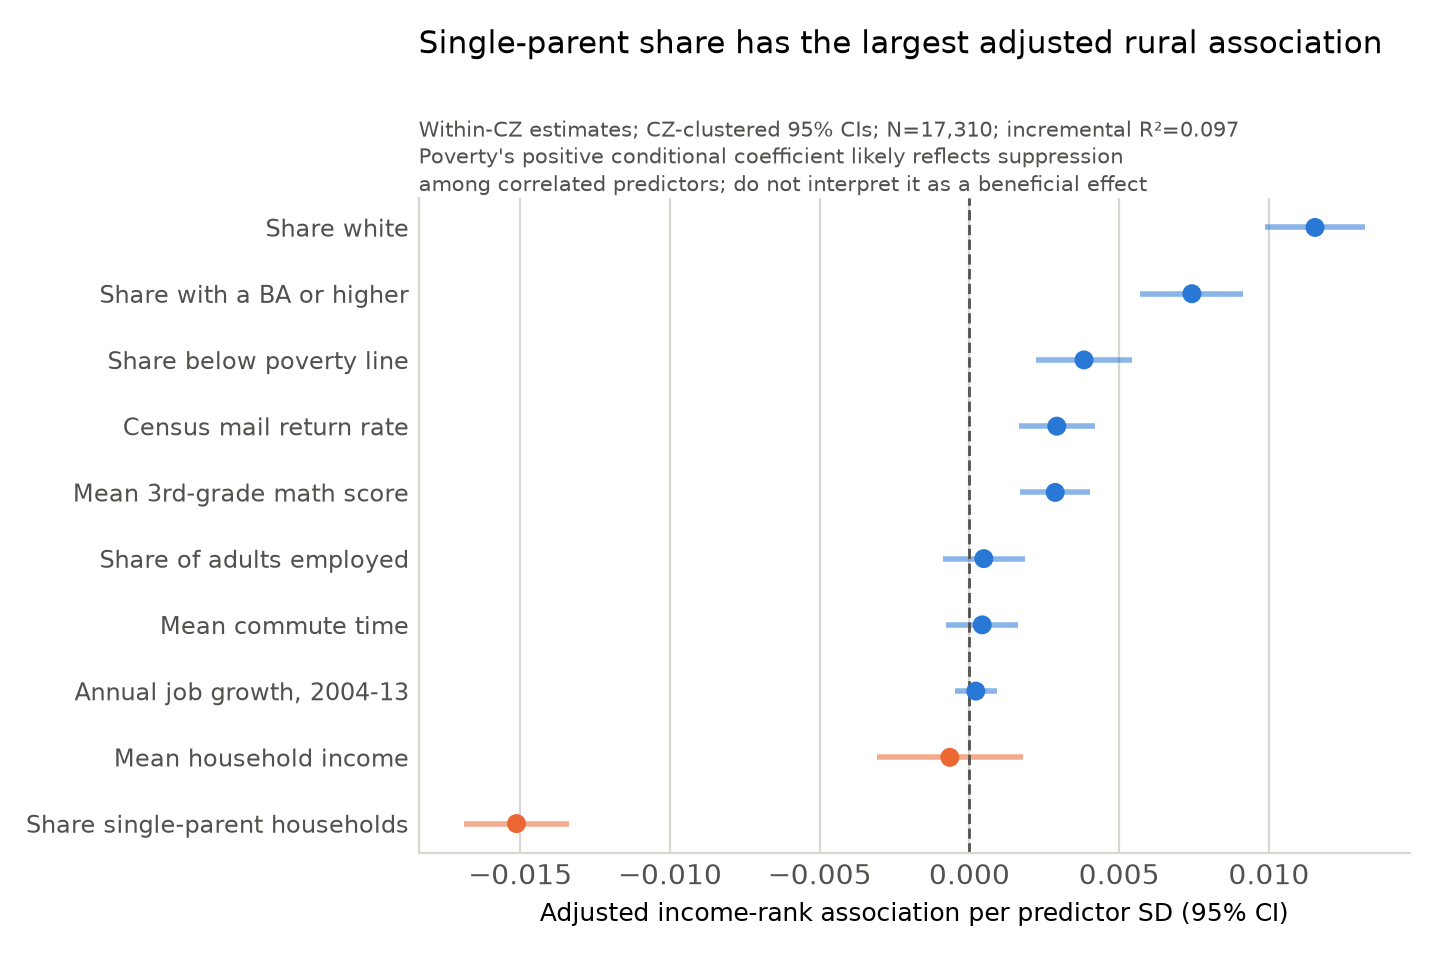
\includegraphics[width=0.73\linewidth]{fig2_rural_ols_coefficients.png}
\caption{\textbf{Single-parent share has the largest adjusted rural
association.} OLS coefficients from Equation~\ref{eq:ols} on 17{,}310 rural
tracts, expressed per standard deviation of each characteristic among rural
tracts, with commuting-zone fixed effects and commuting-zone-clustered 95\%
confidence intervals. Blue denotes positive and orange negative associations.
Job growth, commute time, employment share, and mean household income overlap
zero.}
\label{fig:rural}
\end{figure}

\begin{table}[htbp]
\centering\small
\caption{\textbf{Within-commuting-zone OLS results, rural tracts.}
Coefficients are changes in mean adult household income rank per standard
deviation of each characteristic among rural tracts; multiply by 100 for
percentile points. Confidence intervals are clustered by commuting zone.
$N=17{,}310$ tracts in 727 commuting zones. The reported $R^2$ is the
full-model value and is dominated by the commuting-zone indicators; see the
incremental $R^2$ in the text.}
\label{tab:ols}
\begin{tabular}{lrrr}
\toprule
Characteristic (per SD) & $\beta$ & 95\% CI & $p$ \\
\midrule
Share single-parent households & -0.0271 & [-0.0282, -0.0261] & 0.000 \\
Mean commute time & -0.0109 & [-0.0117, -0.0101] & 0.000 \\
Mean household income & -0.0064 & [-0.0081, -0.0048] & 0.000 \\
Census mail return rate & 0.0008 & [-0.0001, 0.0017] & 0.094 \\
Annual job growth, 2004-13 & 0.0018 & [0.0010, 0.0026] & 0.000 \\
Share below poverty line & 0.0024 & [0.0011, 0.0038] & 0.000 \\
Share of adults employed & 0.0037 & [0.0027, 0.0047] & 0.000 \\
Mean 3rd-grade math score & 0.0039 & [0.0030, 0.0048] & 0.000 \\
Share white & 0.0077 & [0.0066, 0.0087] & 0.000 \\
Share with a BA or higher & 0.0109 & [0.0096, 0.0123] & 0.000 \\
\midrule
N & \multicolumn{3}{r}{17,310} \\
$R^2$ & \multicolumn{3}{r}{0.349} \\
\bottomrule
\end{tabular}

\end{table}

\paragraph{Region explains far more than tract characteristics do.}
Commuting-zone indicators alone account for $R^2=0.564$ of the variation in
rural tract mobility; adding all ten characteristics raises this to 0.661, an
incremental $R^2$ of \textbf{0.097}. These ten characteristics therefore
explain about a tenth of rural mobility variation once region is accounted for.
Most of what predicts a rural child's adult income rank is which regional labor
market they grew up in, not which tract inside it, and reporting the
full-model 0.661 as the covariates' explanatory power would overstate it
roughly sevenfold.

\paragraph{The result survives a precision screen.} Table~\ref{tab:screen}
compares the main coefficients with those from the 14{,}741 rural tracts whose
estimates rest on at least 200 children. Single-parent share is essentially
unchanged and slightly larger ($-0.0151$ to $-0.0157$), as are share white and
third-grade math. Three coefficients change sign: job growth, commute time,
employment share. All three are null in the main model, so these are movements
of noise around zero, not unstable associations; the table marks significance
so this is visible without the surrounding text.

\begin{table}[htbp]
\centering
\caption{\textbf{Sensitivity to a minimum child-count screen.} Main
coefficients (all complete cases, $N=17{,}310$) beside the same model fit only
on tracts whose Atlas estimate rests on at least 200 children
($N=14{,}741$).}
\label{tab:screen}
\footnotesize
\begin{tabular}{lrr}
\toprule
Characteristic & All complete cases & Count $\geq$ 200 \\
\midrule
Share single-parent households & -0.0151 & -0.0157 \\
Mean household income & -0.0007 & -0.0032 \\
Annual job growth, 2004-13 & 0.0002 & -0.0001 \\
Mean commute time & 0.0004 & -0.0002 \\
Share of adults employed & 0.0005 & -0.0005 \\
Mean 3rd-grade math score & 0.0029 & 0.0028 \\
Census mail return rate & 0.0029 & 0.0019 \\
Share below poverty line & 0.0038 & 0.0023 \\
Share with a BA or higher & 0.0074 & 0.0049 \\
Share white & 0.0115 & 0.0114 \\
\bottomrule
\end{tabular}

\end{table}

\paragraph{The rural pattern is not a scaled-down urban one.}
Figure~\ref{fig:compare} places both groups on a common pooled
standard-deviation scale. Single-parent share leads in both settings but is
markedly \emph{stronger} in dense-urban tracts ($-0.031$ versus $-0.021$ per
pooled SD), and share below the poverty line \emph{reverses sign}: positive in
rural tracts ($+0.005$), negative in dense-urban ones ($-0.012$). Mean
household income does the same, near zero in rural tracts and strongly negative
in dense-urban ones ($-0.016$). The positive rural poverty coefficient should
not be read as poverty benefiting children: with mean income, employment, and
single-parent share in the same model, poverty share is heavily collinear with
the other predictors ($r=0.64$ with mean household income, $0.62$ with
single-parent share), and a conditional coefficient that reverses its bivariate
sign here is best understood as suppression among correlated regressors. The
comparison is \textbf{exploratory}: the dense-urban model has only 28
commuting-zone clusters, below the range where cluster-robust standard errors
are reliable~\cite{cameron2015practitioner}, so its intervals are likely too
narrow. It compares shape, not magnitude.

\begin{figure}[htbp]
\centering
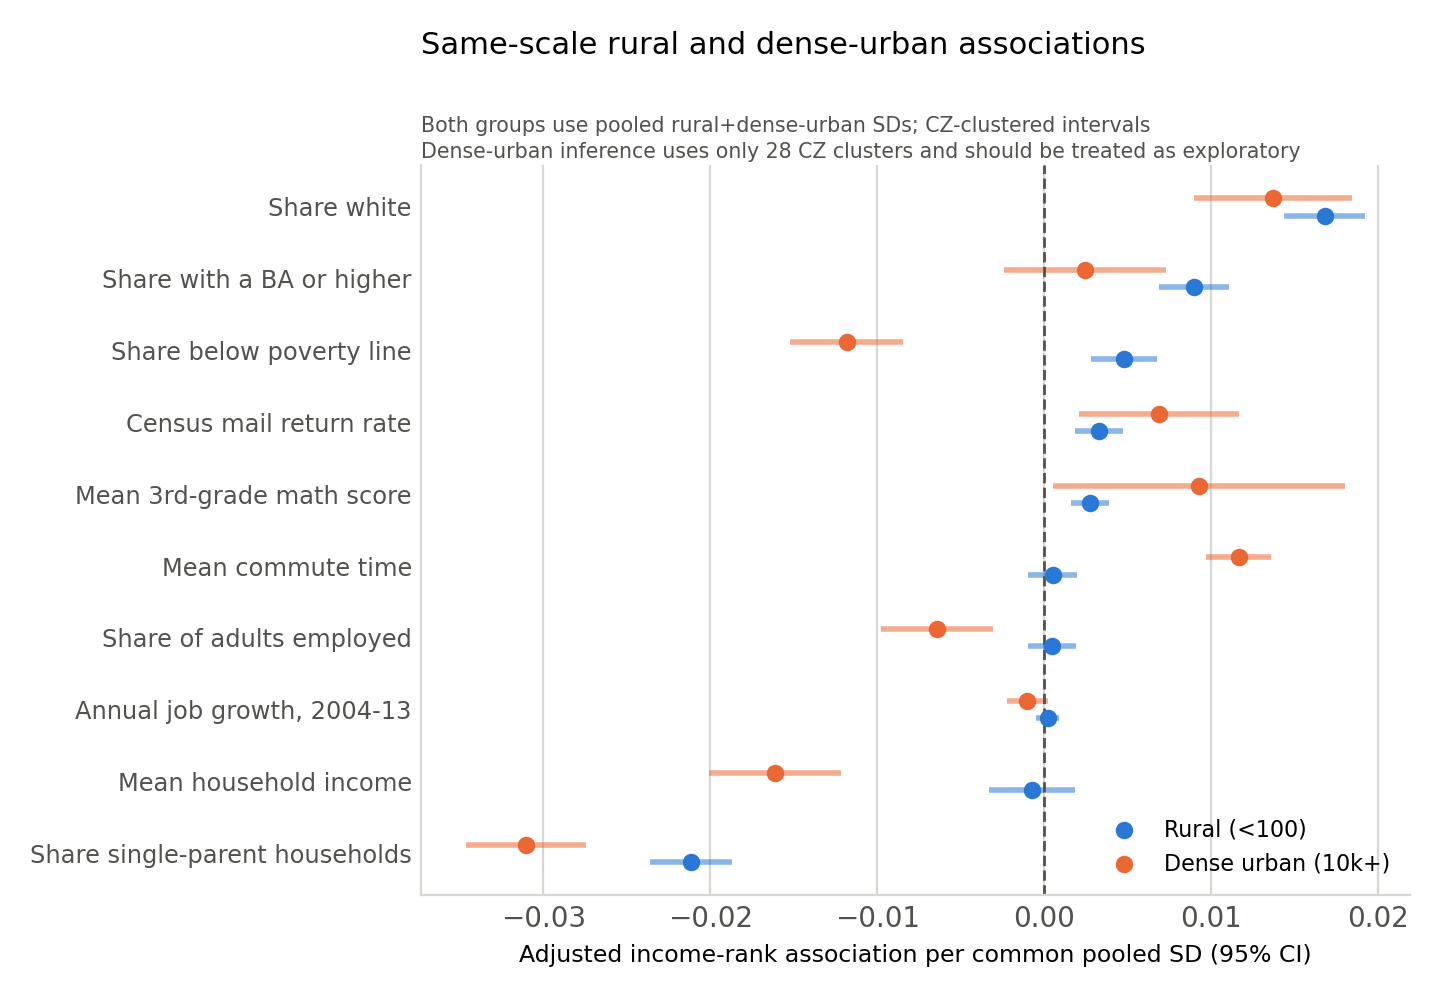
\includegraphics[width=0.73\linewidth]{fig3_rural_dense_coefficients.png}
\caption{\textbf{Same-scale rural and dense-urban associations.} Coefficients
from Equation~\ref{eq:ols} fit separately on rural ($<$100 people per square
mile, $N=17{,}310$, 727 clusters) and dense-urban ($\geq$10{,}000,
$N=2{,}468$, 28 clusters) tracts, both standardized by pooled predictor
standard deviations so the two are directly comparable. Because the scale
differs from Figure~\ref{fig:rural}, the same rural coefficient appears here as
$-0.021$ rather than $-0.015$. Dense-urban intervals rest on 28 clusters and
are exploratory.}
\label{fig:compare}
\end{figure}

%% ====================================================================
\section{Discussion}
%% ====================================================================

Among rural Census tracts in the same commuting zone, single-parent household
share is the largest adjusted correlate of the adult income rank of children
raised in low-income families, and local economic conditions are
indistinguishable from zero. This extends the national cross-commuting-zone
pattern in~\cite{chetty2014land} into rural America and into a
within-labor-market comparison, and it survives a precision screen. It is also
the within-rural counterpart to~\cite{connor2023rural}: they find that
two-parent household share accounts for the rural advantage \emph{over} urban
places, and I find that the same characteristic orders rural tracts against one
another. The second
result is a caution about magnitude: ten tract characteristics add under a
tenth to the variance region alone explains.

Four limitations bound these claims. They are conditional associations, not
effects: the design cannot separate a neighborhood effect from families sorting
into neighborhoods, and single-parent share may proxy for family resources that
travel with children regardless of place. The predictors are strongly collinear
(mean income with BA share, $r=0.78$), so coefficients trade off against one
another and the poverty coefficient is a suppression artifact. ``Rural'' is a
density cutoff of my own choosing, not the Census Bureau's. And the dense-urban
comparison rests on 28 clusters.

The most important finding of this project was the correlation between
single-parent households and mobility, and I think future work on rural
mobility could be targeted towards finding the causes of this correlation, and
other traits associated with the share of single-parent households.

%% ====================================================================
\begin{thebibliography}{99}
\small
\bibitem{chetty2015mto} Chetty, R., Hendren, N., \& Katz, L.~F. (2015).
\textit{The Effects of Exposure to Better Neighborhoods on Children: New
Evidence from the Moving to Opportunity Experiment}. NBER Working Paper
No.~21156.
\bibitem{chetty2017exposure} Chetty, R., \& Hendren, N. (2017). \textit{The
Impacts of Neighborhoods on Intergenerational Mobility I: Childhood Exposure
Effects}. NBER Working Paper No.~23001.
\bibitem{chetty2018county} Chetty, R., \& Hendren, N. (2018). The Impacts of
Neighborhoods on Intergenerational Mobility II: County-Level Estimates.
\textit{The Quarterly Journal of Economics}, 133(3), 1163--1228.
\bibitem{chetty2018atlas} Chetty, R., Friedman, J.~N., Hendren, N., Jones,
M.~R., \& Porter, S.~R. (2018). \textit{The Opportunity Atlas: Mapping the
Childhood Roots of Social Mobility}. NBER Working Paper No.~25147.
\bibitem{chetty2014land} Chetty, R., Hendren, N., Kline, P., \& Saez, E.
(2014). Where is the Land of Opportunity? The Geography of Intergenerational
Mobility in the United States. \textit{The Quarterly Journal of Economics},
129(4), 1553--1623.
\bibitem{chetty2020race} Chetty, R., Hendren, N., Jones, M.~R., \& Porter,
S.~R. (2020). Race and Economic Opportunity in the United States: An
Intergenerational Perspective. \textit{The Quarterly Journal of Economics},
135(2), 711--783.
\bibitem{reardon2011} Reardon, S.~F. (2011). The Widening Academic Achievement
Gap Between the Rich and the Poor. In G.~J. Duncan \& R.~J. Murnane (Eds.),
\textit{Whither Opportunity?} (Ch.~5). Russell Sage Foundation.
\bibitem{reardonbischoff2011} Reardon, S.~F., \& Bischoff, K. (2011). Income
Inequality and Income Segregation. \textit{American Journal of Sociology},
116(4), 1092--1153.
\bibitem{hanushek2006} Hanushek, E.~A., \& Rivkin, S.~G. (2006). \textit{School
Quality and the Black--White Achievement Gap}. NBER Working Paper No.~12651.
\bibitem{cameron2015practitioner} Cameron, A.~C., \& Miller, D.~L. (2015). A
Practitioner's Guide to Cluster-Robust Inference. \textit{Journal of Human
Resources}, 50(2), 317--372.
\bibitem{weber2017rural} Weber, B.~A., Fannin, J.~M., Cordes, S.~M., \&
Johnson, T.~G. (2017). Upward Mobility of Low-Income Youth in Metropolitan,
Micropolitan, and Rural America. \textit{The ANNALS of the American Academy of
Political and Social Science}, 672(1), 103--122.
\bibitem{connor2023rural} Connor, D., Hunter, L., Jang, J., \& Uhl, J. (2023).
Family, Community, and the Rural Social Mobility Advantage. \textit{Research in
Social Stratification and Mobility}, 87, 100844.
\end{thebibliography}

\clearpage
\appendix
%% ====================================================================
\section{Agentic Analysis}

For this project I mainly used Claude Code, and occasionally used OpenAI Codex
to review or challenge the work that Claude had completed. My typical workflow
was to start by giving the assistant the context in detail, including where my
mind was, what I had currently completed, and the project specifications. I
also had my agents keep a markdown file with current progress on the project
and my general tastes as context for the next session. I found the assistants
particularly useful for learning new statistics concepts that I could implement
in my project. When the assistant would implement something, I would check its
work, use another assistant to challenge it, and ask it to explain things it
had implemented that were outside of my knowledge. One specific example of
something I rejected was the slide design for the presentation. My professor
noted that slide 2 was not providing important information. I agreed, then
hand-picked a new figure to put on the slide. I also took this feedback into
account when writing this paper, making sure to not miss the mark and include
information that is irrelevant.

\subsection*{Transcripts}

\begin{itemize}\itemsep2pt
\item Claude: \href{https://docs.google.com/document/d/16tEyKmXsj5zVQupSGv-JQbtHahILT8lN/edit?usp=sharing}{\texttt{agentic\_transcript\_fortner.docx}}
\item ChatGPT: \href{https://docs.google.com/document/d/1VHYOB-BYbF-cUh4MJhan6rHSXbE5qv2O/edit?usp=sharing}{\texttt{qss20\_chat\_transcript.docx}}
\end{itemize}

\end{document}
